\section{Notes en vrac}
\begin{itemize}
    \item Synthèse: 5 à 10 pages. Might be something good to write in english.
    \item Goal: electricity demand modeling, with forecasting for 2030. 
    \item Observer la \textbf{relation entre prix de l'électricité et changement dans la structure des moyens de production} ces dernières années $\to$ besoins de meilleures variables ?? Ou juste regarder le PIB, contrôler pour l'IPC, etc.
    \item \textbf{impact des marchés de l'électricité sur la demande d'électricité} $\to$ on juge que le prix de l'électricité capture l'effet du "marché" ??
\end{itemize}

\subsection{Description}
\begin{enumerate}
    \item Relation économétrique entre les variables. 
    \item Prévision de la variable dépendante.
\end{enumerate}
The given dataset is composed of 6 time series over electricity consumption, GDP, population, inflation, electricity price, climate index. The data is available from 1990 to 2021, with 32 observations. 
% We first tried to find more granular data, \textit{e.g.} quarterly one, but no source could provide electricity information over the 1990-2021 time period (the IAE has been charging for data since january 2025, Eurostat doesn't have reliable french data before 2005)\footnote{For inflation and GDP, we could have used INSEE database, \href{https://www.insee.fr/fr/statistiques/serie/001763852#Telechargement}{here} and \href{https://www.insee.fr/fr/statistiques/8196636?sommaire=8182908#consulter}{there}.}. From this situation, we already know that, dealing low-frequency data, we will not be able to include annual variability in our analysis, which could have been interesting for studying seasonal effects on electricity. We also will not be able to use moving average filter (\textit{e.g.} Hodrick-Prescott) to identify trends, economic cycles, and fluctuations in the GDP.

\subsection{Notes cours C. Doz}

\subsubsection{Univariate time series}
Stationary around a deterministic trend: $X_t = a + bt + Y_t$ where $(Y_t)_t \in Z$ is a stationary process. (Stationarity if esperance and variance does not depend on $t$).

White noise: variance is constant, no autocorrelation, mean is zero.

Wold theorem: any stationary process can be written as a linear combination of white noise. $X_t = m + \sum_{i=0}^{\infty} \psi_i \varepsilon_{t-i}$. \\


Lag operator: $LX_t = X_{t-1}$. Now, if $(X_t)_t$ is a stationary process:
\begin{itemize}
    \item $AR(p)$ process: $X_t = \mu + \sum_{i=1}^{p} \phi_i X_{t-i} + \varepsilon_t$.
    \item Best Linear Forecast of an $AR(p)$ process: $X^*_{t+1\vert t} = \mu + \sum_{i=1}^{p} \phi_i X_{t+1-i} + \varepsilon_t$.
    \item Moving average process $MA(q)$: $X_t = \mu + \varepsilon_t + \sum_{i=1}^{q} \theta_i \varepsilon_{t-i}$.
    \item $ARMA(p, q)$ process: $X_t = \mu + \sum_{i=1}^{p} \phi_i X_{t-i} + \varepsilon_t + \sum_{j=1}^{q} \theta_j \varepsilon_{t-j}$.
    \item \textbf{If $(X_t)_t$ is an $ARMA(p, q)$ process, autocorrelation should tend exponentially to 0 with increasing lags.}
    \item On these processes, the impact of a shock is transitory.
\end{itemize}

\textit{In our case, electricity consumption might not be ARMA processes, so we might not be able to forecast as such... it is to be tested. We have to test which variables can be considered stationary around a deterministic trend.}

Now, if $X_t = \mu + X_{t-1} + \varepsilon_t$ (random walk), we have: 
\begin{itemize}
    \item ARIMA: $(1 - L)^d \Phi(L)X_t = \mu + \theta(L) \varepsilon$
    \item On ARIMA process, the impact of a shock is permanent.
    \item Autocorrelation of $X_t$ don't exponentially tend to 0 with increasing lags.
    \item Identication and estimation of an $ARIMA(p,d,q)$ :
    \begin{enumerate}
    \item choice of d : visual inspection of the estimated
    autocorrelogram + unit root tests (see below).
    \item If $(X_t)_t$ appears to be non-stationary, study $(1-L)X_t$, etc...
    \item Choose the smallest $d$ such that $(1-L)^d X_t$ appears to be stationary.
    \item choice of (p,q) : compute $Y_t = (1-L)^d X_t$ and apply to $Y_t$ the procedure which has been presented for ARMA(p,q).
    Estimate an ARMA model for $Y_t$.
    \end{enumerate}
\end{itemize}

\subsubsection{Multivariate time series}
Let's consider a vector of time series $(X_t)_t$ with $X_t = (X_{1t}, X_{2t}, \ldots, X_{kt})$. We suppose that $(X_t)_t$ is a stationary process. 

Wold theorem: 
If $(X_t)_t$ is a stationary process and $(\varepsilon_t)_t$ is a white noise, then $(X_t)_t$ can be written as a linear combination of $(\varepsilon_t)_t$: $$X_t = m + \sum_{i=0}^{\infty} A_i \varepsilon_{t-i}, \quad A_0 = I, \sum_{i = 1}^\infty A_i < \infty$$ \\

VAR(p): $X_t = \mu + \sum_{i=1}^{p} \Phi_i X_{t-i} + \varepsilon_t \Leftrightarrow  \Phi(L)X_t = \mu + \varepsilon_t$. \\

\textit{It's not clear that IRC is a good variable to include in the VAR model: it does not seem to be an AR(1) process, or at least not with our granularity.}

To do an IRF: Cholesky decomposition to have an orthogonalized impulse response function.

\subsection{Notes Ferrara - Doz}
\begin{enumerate}
    \item Data analysis
    \item Model specification
    \item Parameter estimation
    \item Model validation by tests
    \item Macro use of the model for forecasting and policy analysis
\end{enumerate}

Bootstrap on residuals is valid if the residuals are white noise and the process is stationary. \\

ARDL: $Y_t = \alpha + \sum_{j=1}^m \beta_j X_{t-j} + \sum_{j=1}^m \gamma_j Y_{t-j} + \varepsilon_t$. 

\textbf{The model specification is generally carried out using
information criteria. }
\\

About Structural VAR: Structural shocks are supposed to be white noise processes and orthogonal to each others.

we could use short-run restrictions with Cholesky decomposition, but also Local Projection à la Jordà (2005) or sign (long-run) restrictions à la Uhlig (2005).

\subsection{Regression}
For $n = 32$ observations, $k = 6$ variables, we use the following linear regression model:
\begin{align*}
    \boldsymbol{Y} & = \boldsymbol{X} \boldsymbol{\beta} + \boldsymbol{\varepsilon} \\
    \begin{bmatrix} 
        y_1 \\ y_2 \\ \vdots \\ y_n 
        \end{bmatrix} & = \begin{bmatrix}
        x_{11} & x_{12} & \cdots & x_{1k} \\ 
        x_{21} & x_{22} & \cdots & x_{2k} \\ 
        \vdots & \vdots & \ddots & \vdots \\ 
        x_{n1} & x_{n2} & \cdots & x_{nk} 
        \end{bmatrix} \begin{bmatrix}
        \beta_1 \\ \beta_2 \\ \vdots \\ \beta_k 
        \end{bmatrix} + \begin{bmatrix} 
        \varepsilon_1 \\ \varepsilon_2 \\ \vdots \\ \varepsilon_n \end{bmatrix}
\end{align*}

Ordinary Least Square (OLS) method is used to estimate the coefficients $\boldsymbol{\beta}$. It holds over the following hypothesis:
\begin{enumerate}
    \item More observations than explanatory variables
    \item Absence of multicollinearity $\to$ useful to check if we are using lags.
    \item Explanatory variables rely on data and the error term is random
    \item The expected value of the error term is zero
    \item Errors are not autocorrelated
    \item Errors are homoscedastic
    \item The error term follows a normal distribution
\end{enumerate}

If the hypotheses 4, 5 and 6 are verified, the error term is white noise. The Durbin-Watson test is used to check the absence of autocorrelation. The Breusch-Pagan test is used to check the homoscedasticity of the error term. The Shapiro-Wilk test is used to check the normality of the error term.

The $R^2$ coefficient is used to evaluate the goodness of fit of the model. It measures the proportion of the variance in the dependent variable that is predictable from the independent variables. The adjusted $R^2$ is used to compare the goodness of fit of models with different numbers of variables.

Confidence interval for $\beta_j \in \{\beta_1, \beta_2, \ldots, \beta_k\}$ is given by a Student's t-distribution with $n - k - 1$ degrees of freedom. (\textit{is it useful?}). \\



\subsection{Nos résultats}
\begin{figure}[h]
    \centering
      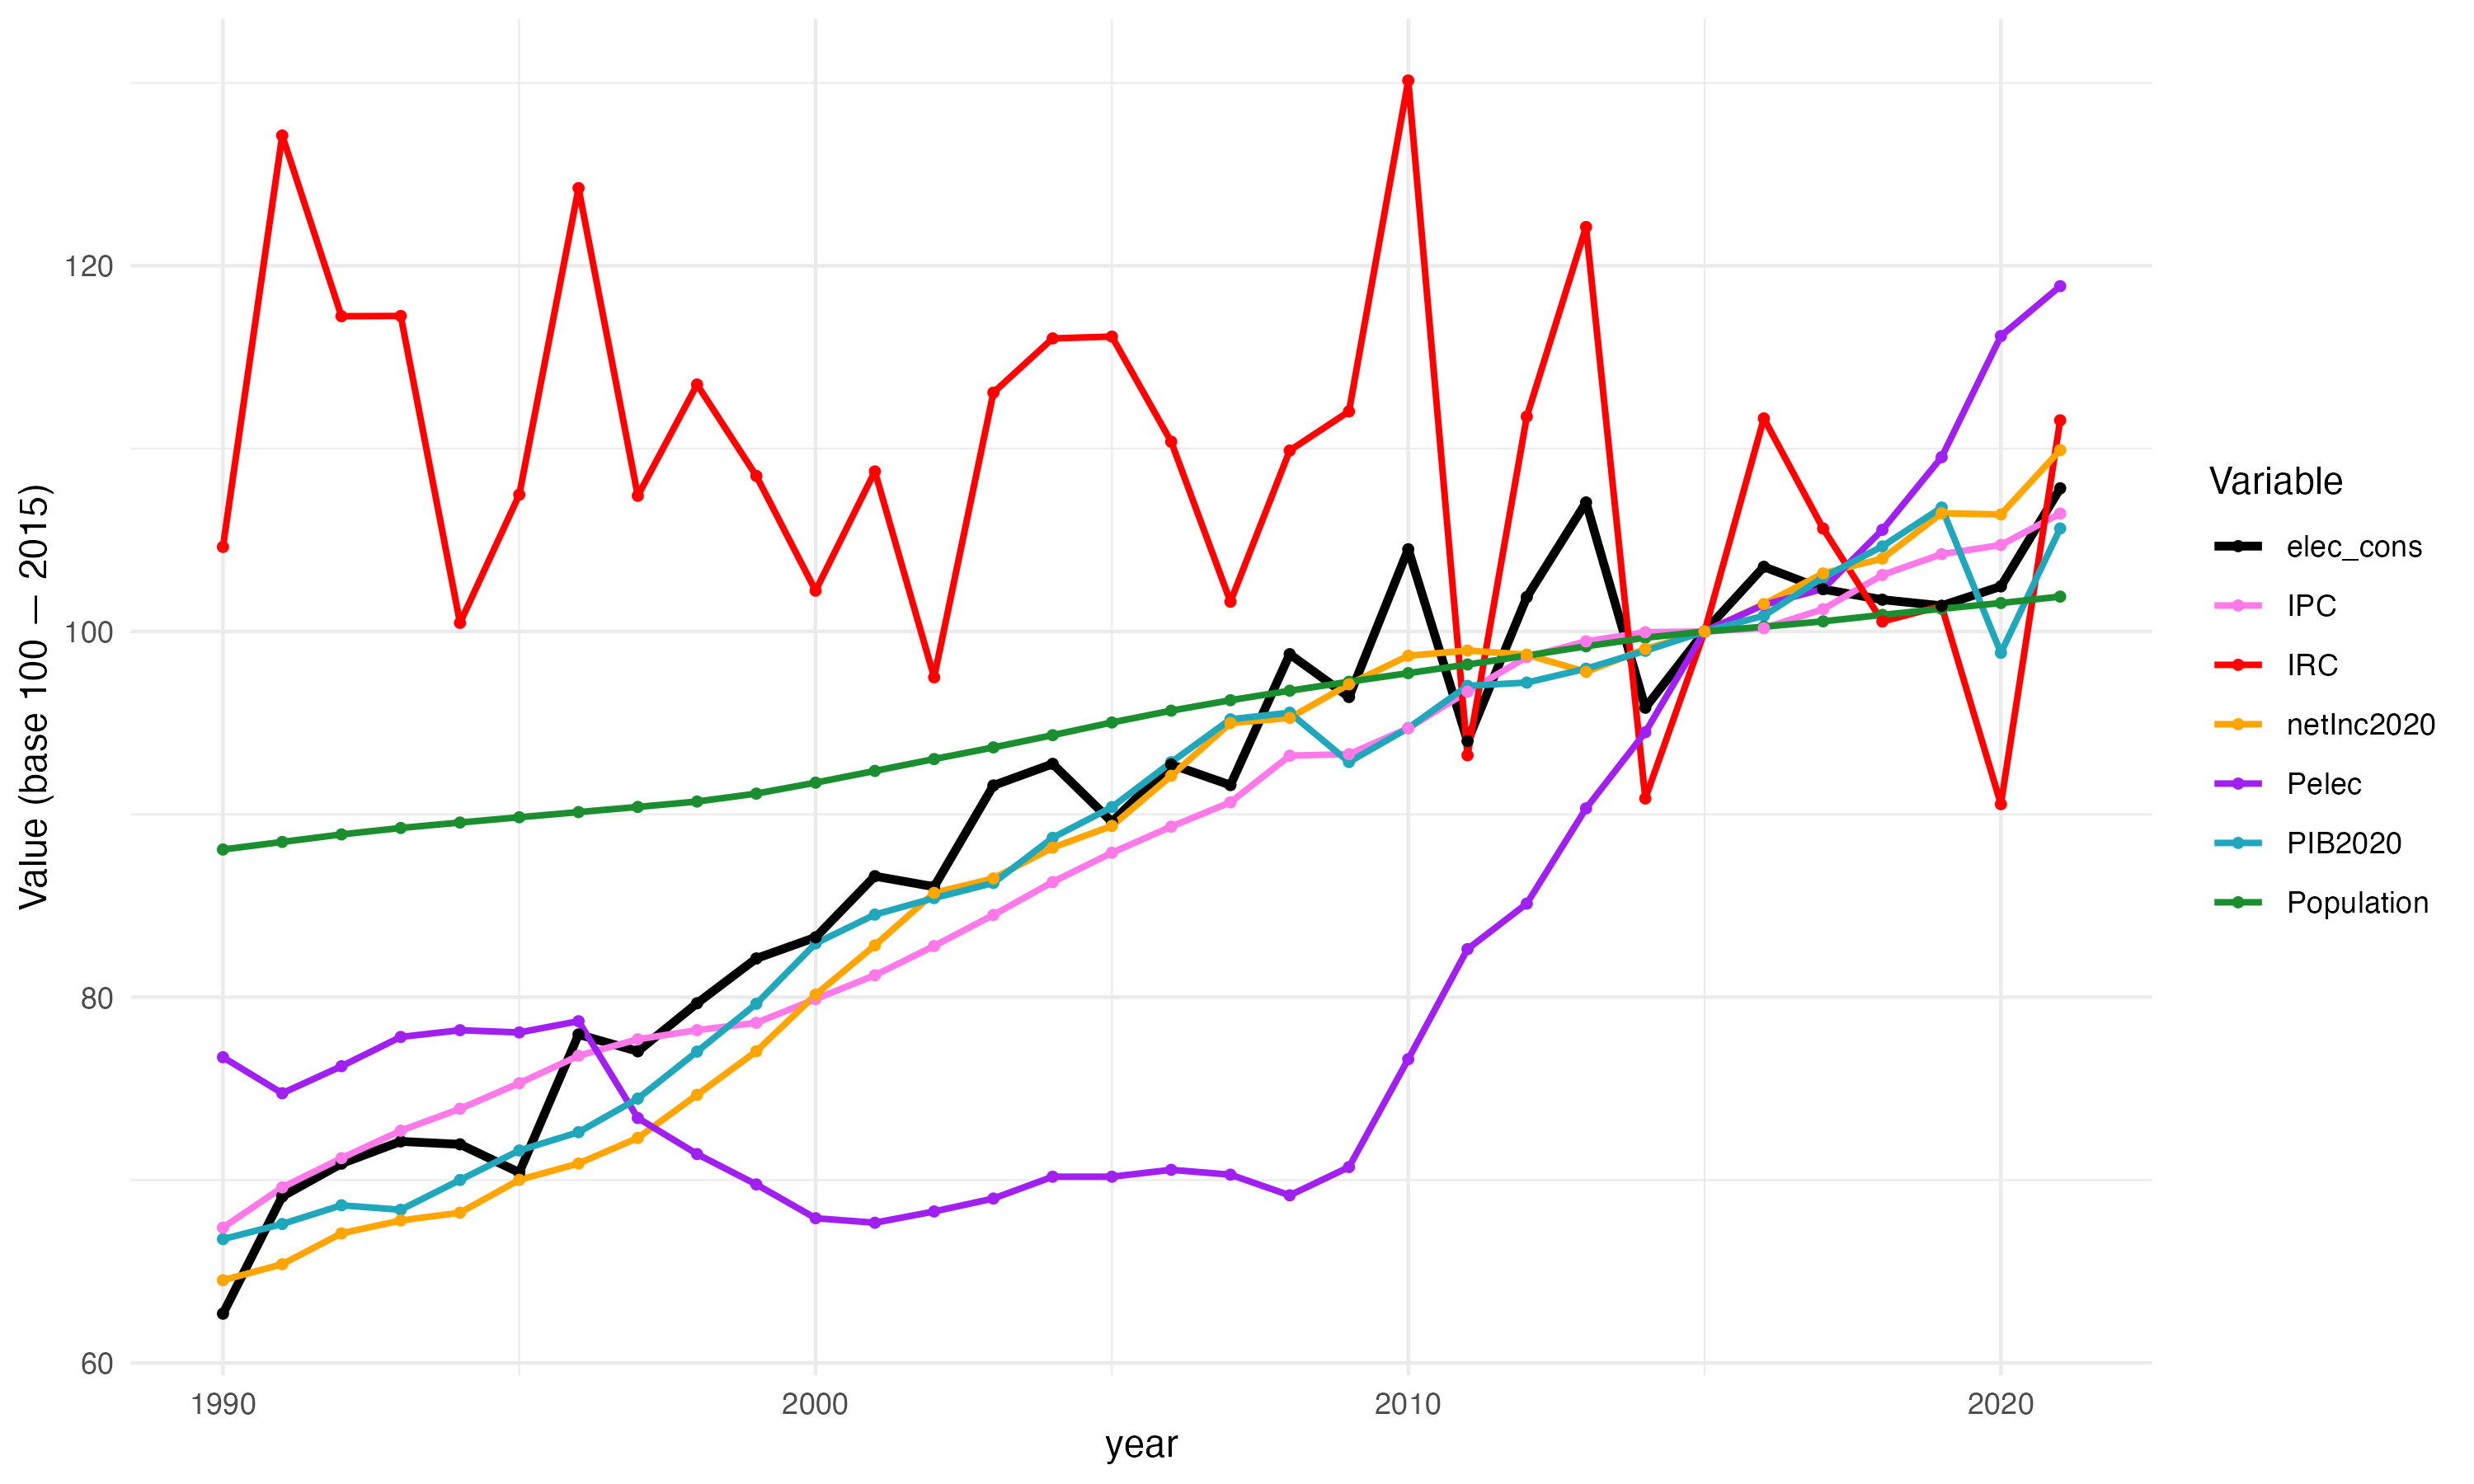
\includegraphics[width=0.54\textwidth]{Images/data_base100_2015.jpeg}
      \caption{Évolution des variables en base 100.}
          \label{var}
  \end{figure}

Graphique 1 : évolution des variables en base 100. On peut déjà intuiter une influence de la croissance du PIB, de la population et de l'indice des prix à la consommation (IPC) sur la demande d'électricité. On remarque aussi comme les fluctuations de l'Indice de Rigueur Climatique (IRC) viennent influencer la consommation d'électricité des ménages. On note enfin que la croissance forte du prix de l'électricité depuis 2009 semble corrélée à la baisse tendancielle du taux de croissance de la consommation d'électricité. Soulignons qu'à partir de cette période, le taux de croissance des prix dépasse celui de l'inflation.

\section{Introduction}
